\chapter{Contribution}
The definition by Binder et al. \cite{binder_definitions_2022} provides a solid foundation for analyzing timing anomalies. However, it does not address branch prediction and related effects. Our goal is to extend this definition to cover such cases. We begin by reviewing Binder's framework and then introduce our own, which supports speculative execution. We describe a new input format that can represent speculative execution, present examples generated by our tool, and discuss how the existing definition can be adapted to these new scenarios.

\section{Methodology}
To systematically investigate timing anomalies induced by branch predictors, it is essential to efficiently generate and analyze relevant examples. Manual construction of such examples is both time-consuming and error-prone, motivating the need for a tool that can automatically or semi-automatically produce and validate them. With such a tool, we can iteratively generate candidate scenarios, analyze their behavior, and assess the applicability of Binder et al.'s definition to these new cases. This process enables us to refine and adapt the definition as necessary, guided by empirical evidence from the generated examples.

Our initial efforts focused on studying and extending the TLA$^+$ \cite{lamport_specifying_2003} framework developed by Binder et al.  to support branch behavior. However, we encountered significant performance limitations and found the input format insufficiently flexible for rapid prototyping and adjustment of examples.

Consequently, we reimplemented the framework in C++, drawing on insights from the TLA$^+$ model. We also use TLA$^+$ as a reference to check the correctness. The new implementation offers substantial performance improvements and introduces randomized search capabilities, enabling efficient exploration of the space of possible instruction traces and facilitating the discovery of timing anomalies related to branch prediction.

\section{Framework}

\subsection{Existing Framework Overview}

\subsubsection{Exploration by Model Checking}

The implementation provided by Binder is written in TLA$^+$ \cite{lamport_specifying_2003}. The pipeline state is specified in set-theory notation. One model checker step corresponds to one clock cycle and derives a new HW state from the previous one. This allows simulation of non-deterministic timing behavior: each time a variation can happen, multiple next states are generated. TLA$^+$ covers all reachable states, ensuring that all possible behaviors are covered.
*
A pair of traces constitutes a whole model state. A TA is expressed as an invariant on pair of traces, so it is verified at each model checking step.

As well as construction of traces, the framework provides visualization methods for the traces and ETDG.

% \TODO{each pair of executions is considered? or all executions are compared against the one reference?}

\subsubsection{Input Trace Format}

The input of the framework is a pair of:
\begin{enumerate}
    \item Pipeline parameters: the superscalar degree, $FU$ latencies, and memory access latencies depending on the cache events (hit or miss).
    \item Instruction sequence: for each instruction, its type and registers are specified, as well as the set of cache behaviors to be explored by the model checker. The type is used to determine which $FU$ will be used by the instruction, and the registers are used to derive the data dependencies.
\end{enumerate}

Figure \ref{fig:TLA-format} illustrates the instruction sequence that causes a TA in Example \ref{ex:simple-ta}. We can simplify this view by directly expressing the resource, dependencies, and possible latencies of each instruction. Figure \ref{fig:input-format} shows the input for the instruction trace from Example \ref{ex:simple-ta}. The first column is the instruction label, the second is the resource used, the third is the set of data dependencies, and the last one captures possible execution latencies. In the same fashion, we could specify variations of latencies for the $IF$ stage, but we skip them for simplicity. This table is sufficient to express a pair of execution traces derived from the instruction trace.

\begin{figure}[H]
\begin{lstlisting}[basicstyle=\fontsize{8}{13}\selectfont\ttfamily]
missLat == 3
mayDMiss == {1}
program == <<
[ ind |-> 1, type |-> "MemRead",  r0 |-> "ra", r1 |-> "",   r2 |-> "", addr |-> "0x1" ],
[ ind |-> 2, type |-> "IntAlu",   r0 |-> "",   r1 |-> "ra", r2 |-> "", addr |-> "0x2" ],
[ ind |-> 3, type |-> "IntAlu",   r0 |-> "rb", r1 |-> "",   r2 |-> "", addr |-> "0x3" ],
[ ind |-> 4, type |-> "MemWrite", r0 |-> "",   r1 |-> "rb", r2 |-> "", addr |-> "0x4" ]
>>
\end{lstlisting}
\caption{TLA$^+$ input format for Binder's framework. Some lines are excluded for brevity}
\label{fig:TLA-format}
\end{figure}


\begin{figure}[htbp]
	\centering
	\begin{tabular}{r|ccc}
    & Resource & Dependencies & Latencies \\ \hline
    \textit{A:} & FU1 &  & $1 | 3$ \\
    \textit{B:} & FU2 & $\{A\}$ & $3$ \\
    \textit{C:} & FU2 &  & $3$ \\
    \textit{D:} & FU1 & $\{C\}$ & $3$ \\
    \end{tabular}

	\caption{Simplified input format of example from Figure \ref{fig:TA1-code}}
	\label{fig:input-format}
\end{figure}

\subsection{Limitations}

Despite using a model checker, the existing framework is capable of exploring only the traces that fit the instruction template. This limits the explored space to what is manually defined by the user. Also, there is no way to express branches and speculative execution.

Nevertheless, the framework may be used to manually specify the instruction trace using a template and generate the resulting pair of execution traces. This allows one to quickly sketch examples and analyze them. Unfortunately, this feature comes with some issues.

The most significant flaw we noticed was the performance. Firstly, TLA$^+$ itself takes a few seconds to generate the initial states of the model. Secondly, the graph is analyzed using a Java embedding, which calls a script in Python that in turn deserializes a graph from the text output of the model checker tool.

Moreover, the input is specified in lengthy TLA$^+$ notation, which prevents fast sketching of examples. Thus, it was decided not to write an extension of the existing framework, but to design a new one from scratch.

\subsection{Our Novel Framework}

We introduce a novel framework inspired by Binder et al., designed to address the limitations of the original implementation. Our framework features a lightweight input format that natively supports branch behavior and speculative execution, enabling concise and intuitive specification of instruction traces. To overcome the performance bottlenecks of TLA$^+$, we implement our solution in C++, providing significant speedup and enabling real-time feedback for rapid prototyping. Also, the performance enhancement allows to explore the larger state spaces effectively. Our framework facilitates efficient analysis of timing anomalies and supports both manual and automated exploration modes.

\subsubsection{Misprediction Region}

The format of the input traces was adapted to handle speculative execution. We decided to use a simplified format as in Figure \ref{fig:input-format} as a baseline. In Binder's framework, the instruction trace format is straightforward: it specifies all instructions that are fetched, executed, and finally committed. In the case of speculative execution, some instructions enter the pipeline but are never committed, being squashed by the resolution of the branch. To tackle this problem, we introduce the notion of the \textit{misprediction region of a branch instruction}.

As an input trace, we specify all instructions that can enter the processor pipeline. As we focus only on the timing behavior of the program, abstracting from memory and register state, we also assume that the control flow is known for a given instruction trace. Thus, for each branch, we may specify the instructions in only one branch in the case of correct prediction. However, in the case of misprediction, the instructions from the incorrect branch are fetched until the branch is resolved. We call such instructions \textit{mispredicted}, and the set of such instructions after the branch a \textit{misprediction region}. 

In our input format, each line describes a single instruction, beginning with the functional unit to be used (\texttt{FU1}, \texttt{FU2}, etc.). This may be followed by an optional label, prefixed with \texttt{\#}. Data dependencies can be specified by listing the labels of dependent instructions, each prefixed with \texttt{@}. Next, the possible execution latencies are provided as a list. For branch instructions, an optional \texttt{*} denotes variation in branch prediction behavior. Misprediction regions are indicated by indentation: an indented instruction belongs to the misprediction region of the most recent less-indented branch instruction. 

Figures \ref{fig:spec-input-ugly} and \ref{fig:spec-input-pretty} present an example of the input format. Figure \ref{fig:spec-input-ugly} displays the raw input as understood by the framework, while Figure \ref{fig:spec-input-pretty} provides a more readable, tabular representation that will be used throughout the remainder of this article. In this example, instructions $C$ and $D$ reside within the misprediction region of instruction $B$. Figure \ref{fig:mispred-intro} illustrates the two possible execution traces derived from this instruction trace: trace $\alpha$ corresponds to correct branch prediction, where $C$ and $D$ are skipped and never enter the pipeline; trace $\beta$ demonstrates the misprediction scenario, in which $C$ and $D$ are fetched but subsequently squashed from the pipeline at clock cycle 5.


\begin{figure}[H]
    \centering
    \begin{subfigure}[b]{0.45\textwidth}
        \centering
\begin{lstlisting}
FU1	 #1	[4]
FU2	 @1	[1] *
    FU2 [4]
    FU2 [4]
FU2		[4]
\end{lstlisting}
        \caption{Input format understandable for framework}
        \label{fig:spec-input-ugly}
    \end{subfigure}
    \hfill
    \begin{subfigure}[b]{0.45\textwidth}
        \centering
\begin{tabular}{rr|ccc}
 &  & Res & Dep. & Lat. \\ \hline
\textit{A:} &  & FU1 &  & $4$ \\
\textit{*B:} &  & FU2 & $\{A\}$ & $1$ \\
& \textit{C:} & FU2 &  & $4$ \\
& \textit{D:} & FU2 &  & $4$ \\
\textit{E:} &  & FU2 &  & $4$ \\
\end{tabular}
        \caption{Input format used further in the text}
        \label{fig:spec-input-pretty}
    \end{subfigure}
    \caption{Two equivalent representations of input format supporting speculative execution}
    \label{fig:two-repr}
\end{figure}



\begin{figure}[H]
	\centering
	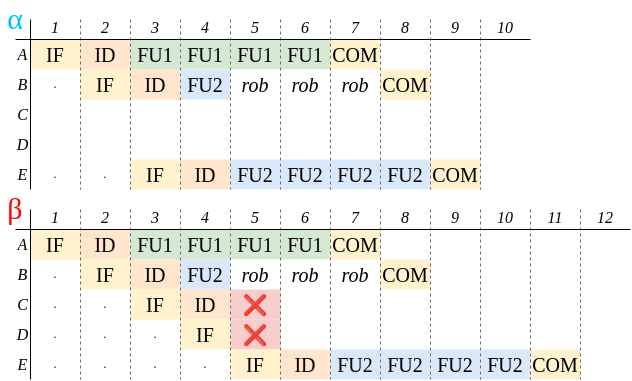
\includegraphics[width=0.6\textwidth]{figures/mispred-intro.png}
	\caption{Pair of traces with correct and incorrect predictions. The squashing event is denoted with a red cross.}
	\label{fig:mispred-intro}
\end{figure}

\TODO{nested mispred region}

\TODO{,ispred region should be sufficiently large}

\subsubsection{Framework Implementation}

We decided to use C++ \cite{stroustrup_c_2015} as the implementation language, as it is fast and includes a number of useful data structures in the standard library.

We define a single instruction as follows. It consists of the type of FU to be scheduled at (we do not consider resource switching), the latency in this FU, and a set of RAW dependencies. If the instruction is a branch, \texttt{mispred\_region} is set to a positive $n$, denoting that the next $n$ instructions are in the misprediction region of the current instruction. In case of no-branch instructions \texttt{mispred\_region} is set to $0$. If we want to model only the correct prediction, then \texttt{mispred\_region} is set to 0; in this way, the branch behaves as an ordinary instruction. The \texttt{br\_pred} flag specifies if the prediction is correct, which is needed when generating a pair of traces with variation in branch behavior.

\begin{lstlisting}[language=C]
struct Instr {
    int 			fu_type = 0;
    int 			lat_fu = 1;
    std::set<int> 	data_deps;
    int 			mispred_region = 0;
    bool 			br_pred = false;
};
\end{lstlisting}

At the core of our framework is the \texttt{PipelineState} structure, which models the state of all pipeline stages. The \texttt{executed} set tracks instructions that have completed execution in the functional units, enabling dependency resolution. The \texttt{branch\_stack} maintains the context for misprediction regions: each time a branch is fetched, it is pushed onto the stack and remains there until resolved. Together with the \texttt{squashed} set, this mechanism ensures correct handling of mispredicted regions. For simplicity, we do not impose capacity limits on the reservation stations (RS) or reorder buffer (ROB). The \texttt{next()} function advances the pipeline state by one clock cycle and returns whether execution has completed. It operates on the instruction sequence, which is accessed via the program counter (\texttt{pc}).

To obtain an execution trace from a given instruction sequence, we initialize an empty pipeline state (with no instructions present) and repeatedly call \texttt{next()} until the final state is reached. This process yields a sequence of pipeline states, which together form an execution trace.

\begin{lstlisting}[language=C]
struct StageEntry {
    int idx = -1;
    int cycles_left = 0;
};

struct PipelineState {
    int clock_cycle = 0;
    int pc = 0;
    vector<StageEntry> 	stage_IF = 	vector<StageEntry>(SUPERSCALAR);
    vector<int> 		stage_ID = 	vector<int>(SUPERSCALAR);
    vector<set<int>> 	stage_RS = 	vector<set<int>>(FU_NUM);
    vector<StageEntry> 	stage_FU = 	vector<StageEntry>(FU_NUM);
    vector<int> 		stage_COM = vector<int>(SUPERSCALAR);
    deque<int> 			ROB = 		deque<int>();
    set<int> 	executed;
    set<int> 	squashed;
    vector<int> branch_stack;

    bool next(const vector<Instr>& prog);
};
\end{lstlisting}

To enable efficient exploration of trace pairs that demonstrate timing anomalies (TA) and to support analysis over larger state spaces, not limited to a fixed instruction trace template, the framework provides three operating modes:

\begin{enumerate}
	\item \textbf{Manual mode}: The user provides an instruction trace in the format given above. The framework then generates the corresponding pair of execution traces. This mode enables rapid construction and analysis of custom scenarios.
	\item \textbf{Random search}: The framework generates random instruction traces within user-defined constraints and checks the resulting execution traces against a specified property. For example, it can explore all traces of length 5 containing one branch instruction and at most two RAW dependencies. While this method cannot guarantee exhaustive coverage of the state space, it is effective for quickly finding counterexamples in large spaces.
	\item \textbf{State exploration}: The trace template is specified as a generator function, similar to random search mode. The framework then exhaustively verifies the property on every possible input, ensuring complete state space coverage. This mode is useful for proving properties about the model, but may be inefficient for finding counterexamples in large spaces due to the potential for excessive exploration of uninteresting subspaces.
\end{enumerate}


In summary, we created a tool capable of studying traces both in automated and guided way. Our time-efficient implementation enables exploration of significantly larger state spaces that are infeasible to analyze using Binder's original framework. While TLA$^+$ offers greater expressive power for formalizing properties such as leveraging temporal logic, in the context of Binder et al., the verified property was ultimately specified as a state predicate embedded in Python code. Therefore, we believe that our choice of implementation does not result in a substantial loss of expressiveness or rigor for the intended analyses.

\section{Generating TA Examples}

We begin by generating representative examples of branch-induced timing anomalies (TAs). Our working hypothesis is that correct branch prediction can, in certain scenarios, result in longer execution times compared to cases with misprediction. To obtain minimal and illustrative examples, we perform an exhaustive search over the space of programs characterized by the following constraints:

\begin{enumerate}
    \item 4 committed instructions with;
    \item At most 2 dependencies;
    \item 1 branch instruction.
\end{enumerate}

The latency of the branch instruction was set to $1$, reflecting the fact that conditional jumps typically involve simple, single-cycle operations (e.g., equality, greater-than-or-equal, less-than-or-equal comparisons). The Latency of all other instructions in this setting was set to $4$. We considered a single-issue pipeline equipped with two functional units. Our framework explored $4608$ input traces in approximately $150$ ms, identifying two timing anomalies, as detailed in Examples \ref{ex:bp-ta} and \ref{ex:bp-ta-1}.

\begin{example}
Figure \ref{fig:bp-ta-inputs-0} presents an instruction trace identified through random example generation. Here, $C$ is a branch instruction with a misprediction region comprising $\{D, E\}$. The only data dependency is $A \rightarrow B$. The corresponding pair of execution traces is depicted in Figure \ref{fig:bp-ta-traces-0}. In trace $\alpha$, instructions $D$ and $E$ are skipped due to correct branch prediction, allowing $F$ to be fetched immediately. This results in $F$ executing earlier and occupying $FU2$ at clock cycle $7$, which in turn delays the execution of instruction $B$ and leads to an overall slowdown.

\label{ex:bp-ta}
\end{example}

\begin{example}
The second timing anomaly, illustrated in Figures \ref{fig:bp-ta-inputs-1} and \ref{fig:bp-ta-traces-1}, differs from Example \ref{ex:bp-ta} only in the functional unit assigned to instruction $C$; all other instructions remain unchanged. Additionally, the misprediction region is extended due to the increased delay between branch prediction and branch resolution.
\label{ex:bp-ta-1}
\end{example}


\begin{figure}
    \centering
    \begin{subfigure}[b]{0.45\textwidth}
        \centering
        \begin{tabular}{rr|ccc}
            &  & Res. & Dep. & Lat. \\ \hline
            \textit{A:} &  & FU1 &  & $4$ \\
            \textit{B:} &  & FU2 & $\{A\}$ & $4$ \\
            \textit{*C:} &  & \textbf{FU2} &  & $1$ \\
            & \textit{D:} & FU1 &  & $4$ \\
            & \textit{E:} & FU1 &  & $4$ \\
            \textit{H:} &  & FU2 &  & $4$ \\
        \end{tabular}
        \caption{Input from Example \ref{ex:bp-ta}}
        \label{fig:bp-ta-inputs-0}
    \end{subfigure}
    \hfill
    \begin{subfigure}[b]{0.45\textwidth}
        \centering
        
        \begin{tabular}{rr|ccc}
            &  & Res. & Dep. & Lat. \\ \hline
            \textit{A:} &  & FU1 &  & $4$ \\
            \textit{B:} &  & FU2 & $\{A\}$ & $4$ \\
            \textit{*C:} &  & \textbf{FU1} &  & $1$ \\
            & \textit{D:} & FU1 &  & $4$ \\
            & \textit{E:} & FU1 &  & $4$ \\
            & \textit{F:} & FU1 &  & $4$ \\
            & \textit{G:} & FU1 &  & $4$ \\
            \textit{H:} &  & FU2 &  & $4$ \\
        \end{tabular}
        \caption{Input from Example \ref{ex:bp-ta-1}}
        \label{fig:bp-ta-inputs-1}
    \end{subfigure}
    \caption{Two anomalous inputs found from the setting}
    \label{fig:bp-ta-inputs}
\end{figure}



\begin{figure}
    \centering
    \begin{subfigure}[b]{0.49\textwidth}
        \centering
        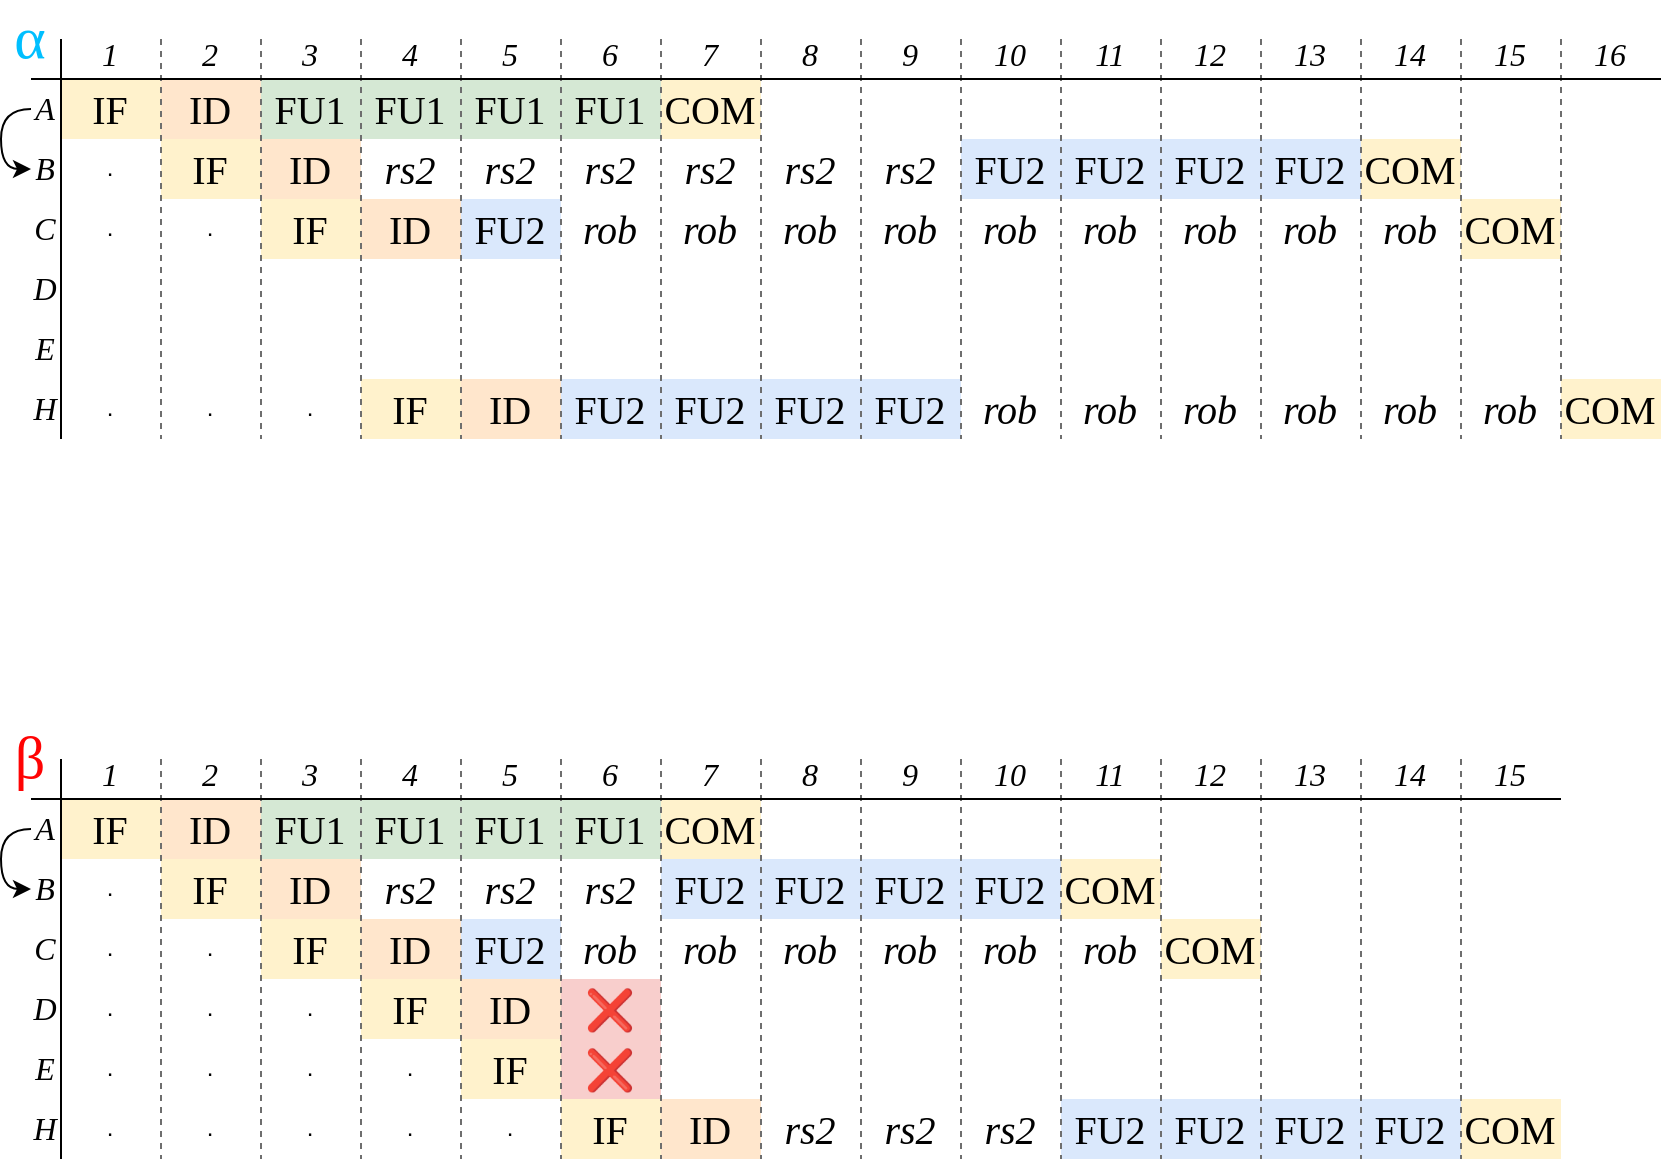
\includegraphics[width=\textwidth]{figures/simple-branch-ta.png}
        \caption{Trace from Example \ref{ex:bp-ta}}
        \label{fig:bp-ta-traces-0}
    \end{subfigure}
    \hfill
    \begin{subfigure}[b]{0.49\textwidth}
        \centering
        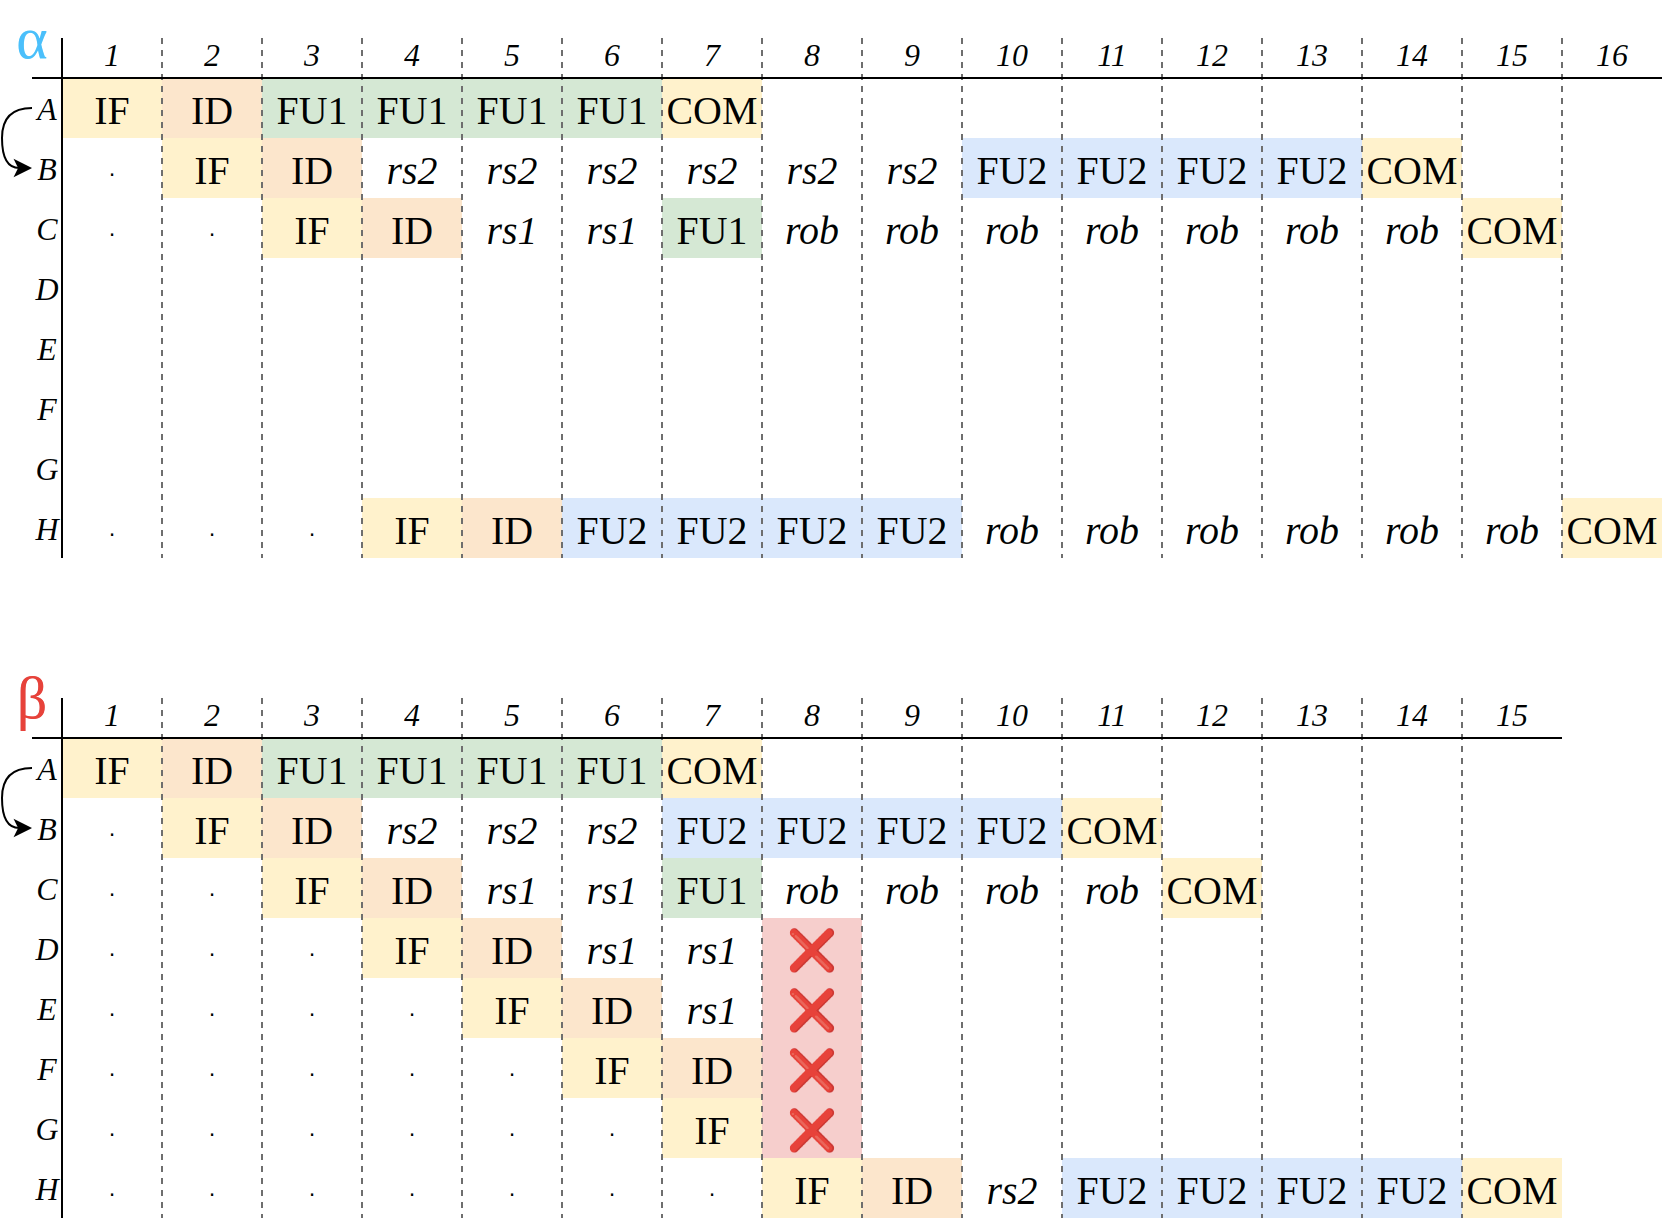
\includegraphics[width=\textwidth]{figures/simple-branch-ta-1.png}
        \caption{Trace from Example \ref{ex:bp-ta-1}}
        \label{fig:bp-ta-traces-1}
    \end{subfigure}
    \caption{Two TA traces found by the framework}
    \label{fig:bp-ta-traces}
\end{figure}

The only essential difference between Examples \ref{ex:bp-ta} and \ref{ex:bp-ta-1} is the length of the misprediction region. The scheduling of instructions $A$, $B$, and $H$ remains identical in both examples. This suggests that certain anomalies may share underlying mechanisms, potentially enabling a classification of timing anomalies (TAs) based on their structural similarities.

Another notable observation is that, in these cases, the anomalous effect can be attributed solely to the delayed fetch of instruction $H$. Remarkably, an equivalent effect can be reproduced by introducing a cache miss during the fetch of $H$, as illustrated in Figure \ref{fig:equiv-to-bp-ta}. In this scenario, both $\alpha$ and $\beta$ traces feature correct branch prediction; however, a cache hit occurs in $\alpha$, while a cache miss occurs in $\beta$. This equivalence may help us to adapt the existing definition.

\TODO{TA only on commit; no longer effect?}

\begin{figure}[H]
    \centering
    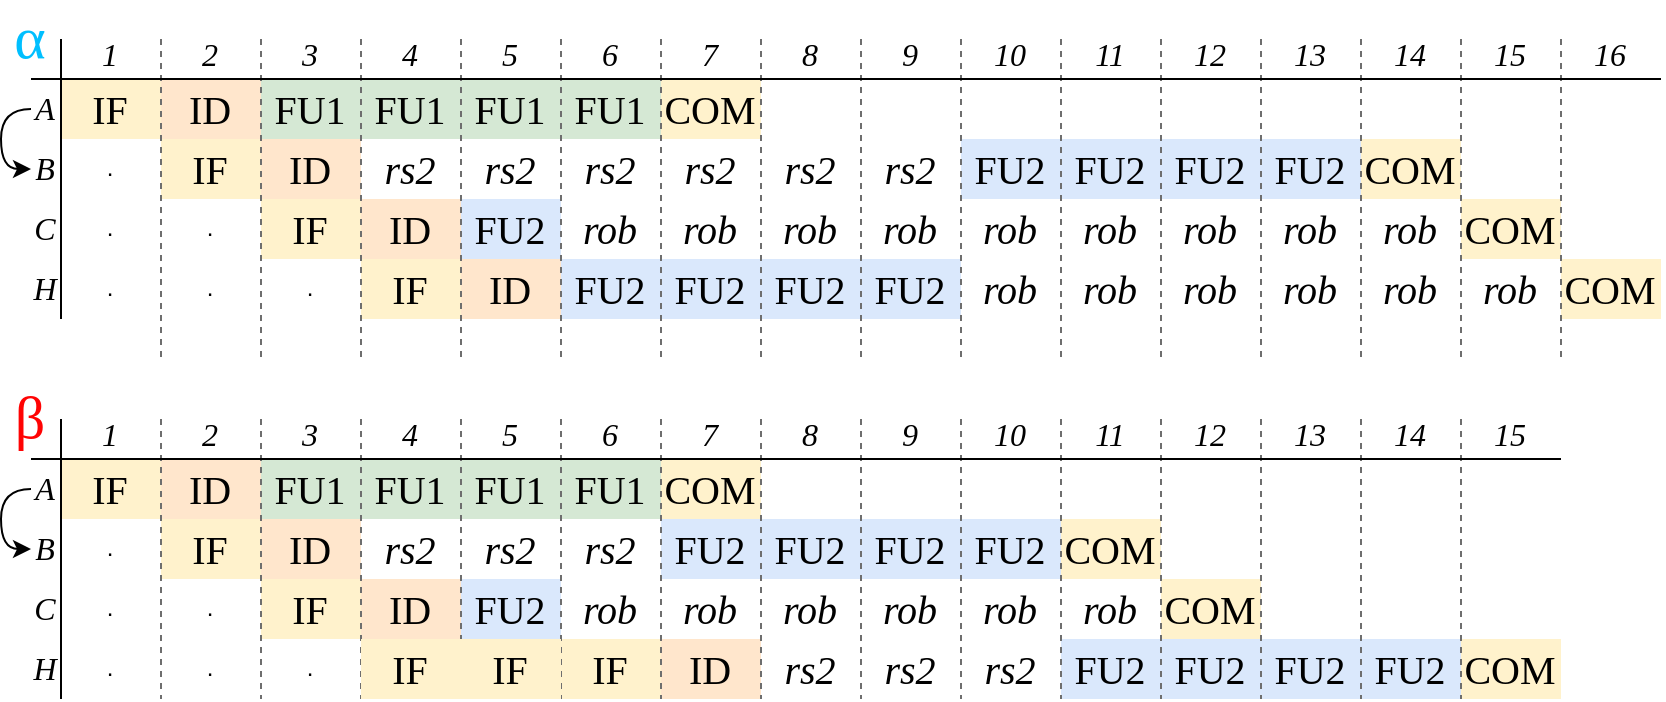
\includegraphics[width=\textwidth]{figures/equiv-trace.png}
    \caption{Cache miss on fetch of $H$ causing the same effect as branch misprediction}
    \label{fig:equiv-to-bp-ta}
\end{figure}

\section{Formalizing TA Definition}

Given that, for the Examples \ref{ex:bp-ta} and \ref{ex:bp-ta-1}, there exists an equivalent scenario without branches in which the timing anomaly can be explained by Binder's definition (see Figure \ref{fig:equiv-to-bp-ta}), it appears feasible to apply the same definition to branch-related cases with minimal modification.


To adapt the existing definition in the context of branch predictors, we start by defining a variation, which is the source of a TA and therefore should be understood first. First, let us consider the trace illustrating the equivalent behavior (Figure \ref{fig:equiv-to-bp-ta}) to Example \ref{ex:bp-ta}, where the variation occurs in the IF latency, i.e., the delay between $\IFa_H$ and $\IFr_H$. In Example \ref{ex:bp-ta}, the event $\IFr_H$ has the same positions in traces $\alpha/\beta$ as in the equivalent trace (Figure \ref{fig:equiv-to-bp-ta}), so it can be used as the end of the variation. But for the start of the variation, $\IFa_H$ cannot be used in the case of branching, as $\IFa_H$ moves along with $\IFr_H$, keeping the same delay. Notably, in Binder's framework, for a given instruction, $\IFa$ coincides with the $\IFr$ of the preceding instruction. This means that we can use $\IFa$ and $\IFr$ of consecutive instructions interchangeably during latency definition. Therefore, the latency can be measured between the $\IFr$ of the branch instruction and the $\IFr$ of the first instruction following the misprediction region.

However, it is important to account for other variations that may occur concurrently, as variations in the IF stage of the post-branch instruction can overlap with branch-related variations, potentially confounding their respective latencies. To address this, we propose marking two distinct events to capture the variation:


\begin{enumerate}
    \item \textbf{Branch Prediction (BP)} -- the moment when the prediction occurs and speculative execution starts;
    \item \textbf{Correct Branch Taken (BT)} -- the instruction from the correct branch enters the pipeline.
\end{enumerate}

Note that $BP$ corresponds to the $\IFr$ of the branch instruction and $BT$ is the $\IFa$ of the first instruction after the misprediction region of the branch. In the case of a single variation that is in branch prediction, the TA pattern is detected in the same way as shown in Figure \ref{fig:equiv-to-bp-ta}, but with the latency being shorter by one clock cycle and the delay being longer by the same value.

Figure \ref{fig:bp-ta-analyzed} shows this idea applied to Example \ref{ex:bp-ta}. Both latencies corresponding to the variation are one clock cycle shorter compared to the example shown in Figure \ref{fig:equiv-to-bp-ta}. The causality region also starts one clock cycle earlier; however, it still goes through the same events. Note here that we do not need any additional rules to build causality arcs.

\begin{figure}
    \centering
    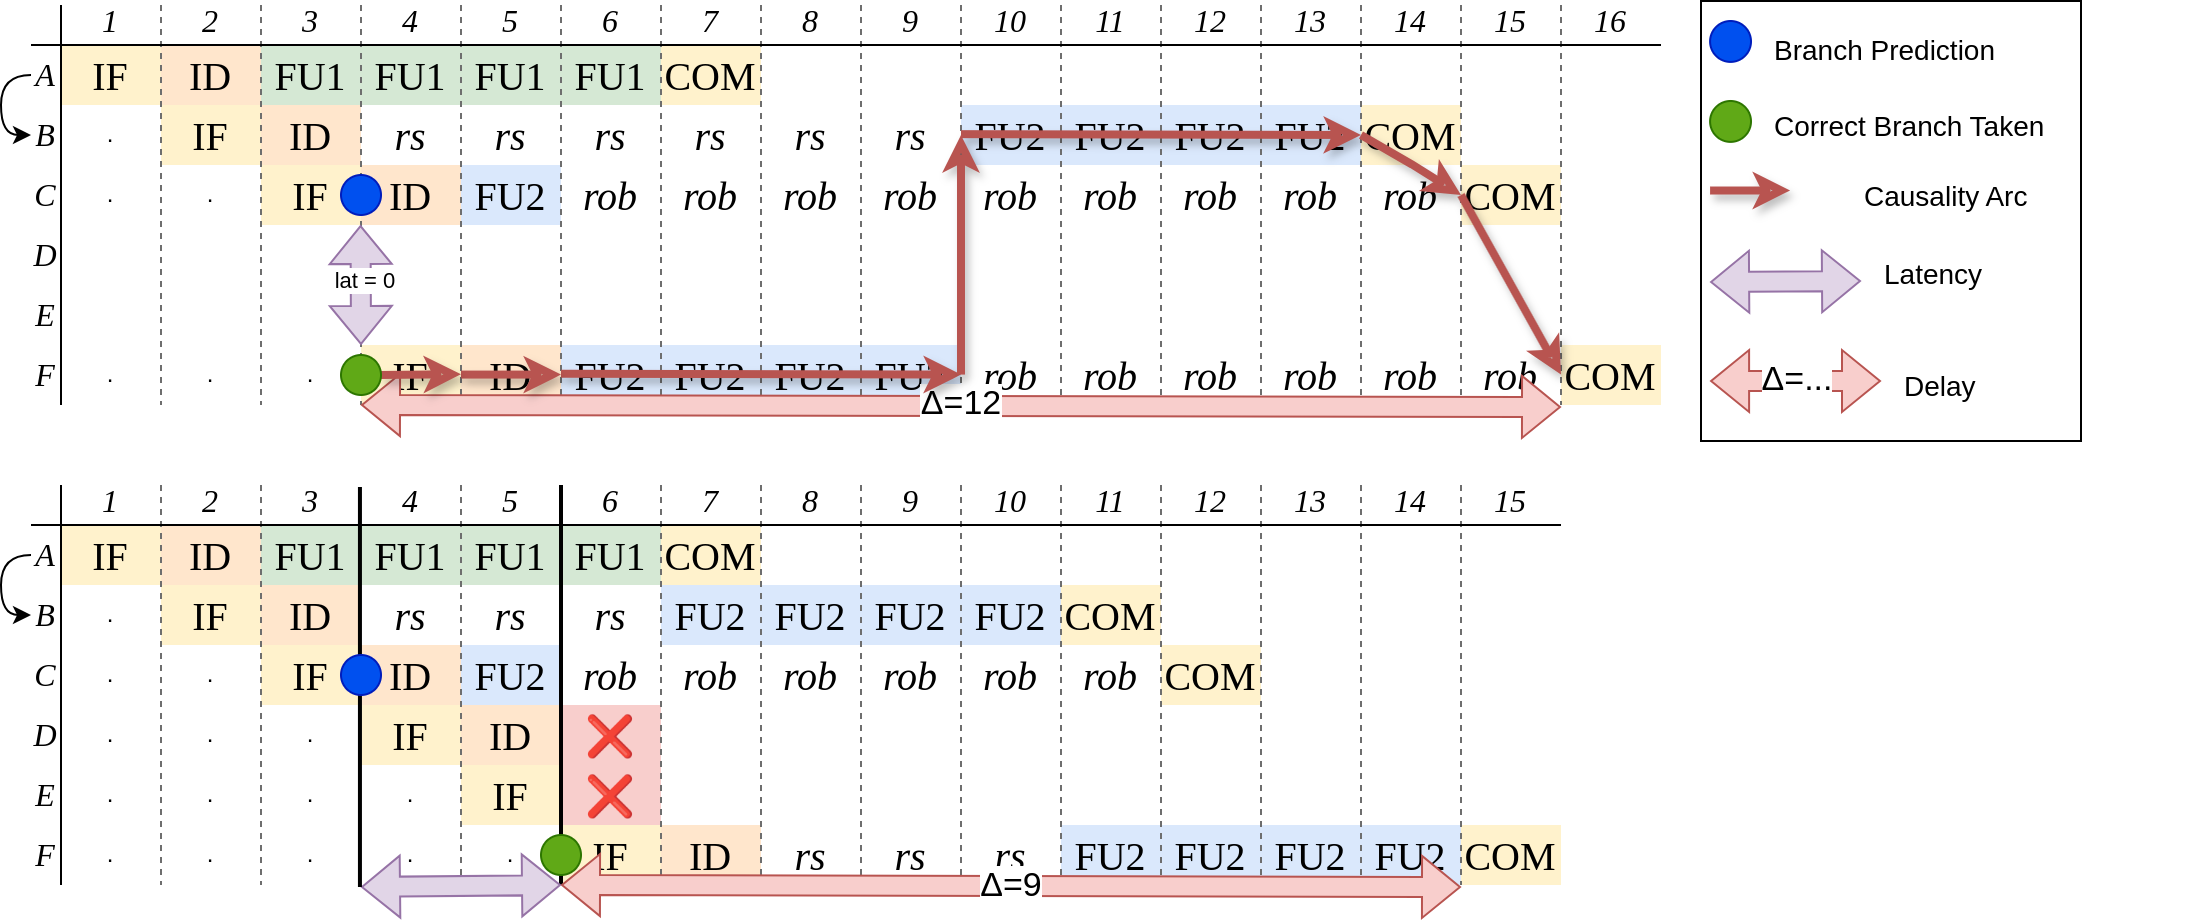
\includegraphics[width=\textwidth]{figures/simple-branch-ta-analyzed.png}
    \caption{The new TA-definition applied to Example \ref{ex:bp-ta}}
    \label{fig:bp-ta-analyzed}
\end{figure}

A major assumption that allowed us to adapt the definition is that the branch behavior is just postponing the fetch of the instruction following the misprediction region. In this case, the behavior can be compared to the effect of a cache miss in the IF stage. This is also not completely true, as the penalty for a cache miss is fixed, while the size of the misprediction region depends on the time between the prediction and the resolution of the branch. Therefore, in the rest of the article, we focus more on examples that do not fit this assumption.

\TODO{Bound the effect of branch resolution?}

\TODO{Conclusion: definition somehow works, but we need to study its limitations}



\section{Limitations of the Definition}

So far, we have demonstrated the potential of using Binder's definition in detecting branch prediction-related TAs. Now we discuss the limitations of the method by providing relevant examples. We start by describing a problem, which appears within the existing framework and is not even related to branch prediction. Then we give more complex examples of branch prediction-caused TAs and try to reason whether they exhibit the same type of flaw or introduce new issues.

\subsection{Gap Problem}

\begin{figure}[H]
    \centering
    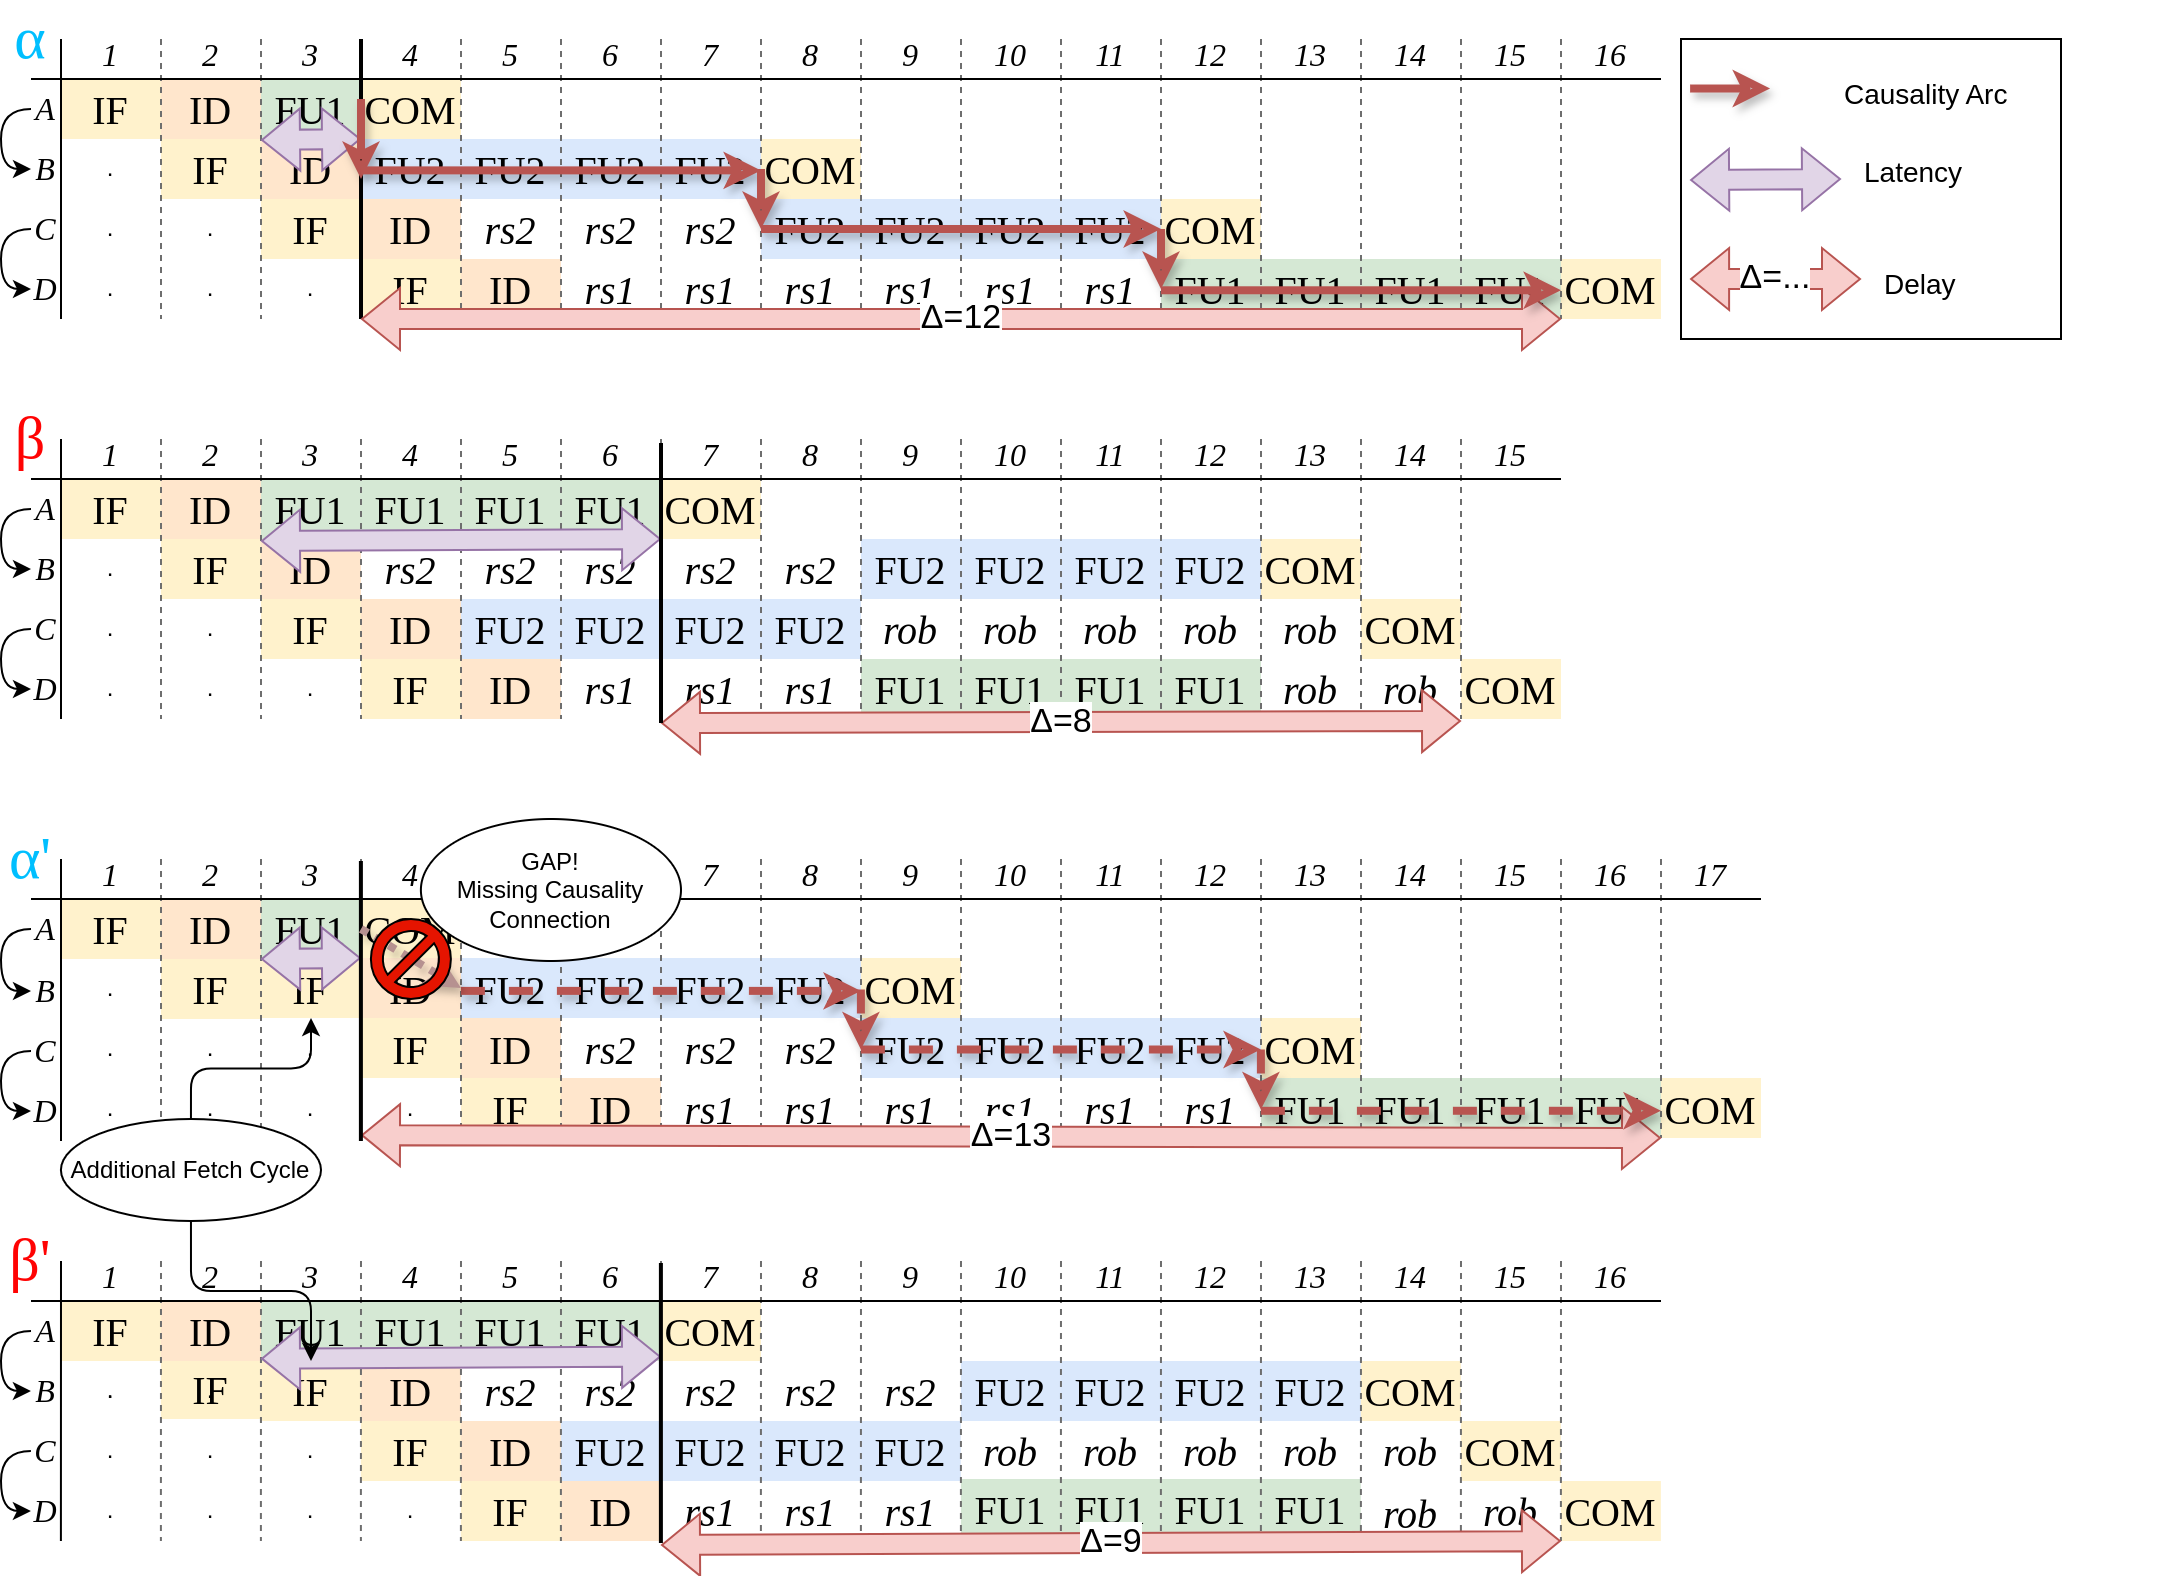
\includegraphics[width=\textwidth]{figures/gap-problem.png}
    \caption{Gap problem}
    \label{fig:gap-problem}
\end{figure}

While testing the existing definition using the framework made by Binder et al., we encountered a situation where a TA clearly exists but is not captured by the framework. We called such an issue the \textit{gap problem}. Figure \ref{fig:gap-problem} shows an example of such a problem: the pair of traces $\alpha/\beta$ shows an example of a TA similar to the one seen in Example \ref{ex:simple-ta}; Binder's definition works fine for this pair. In the pair of traces $\alpha'/\beta'$, we change the latency for the fetch of instruction $B$. This creates a so-called \textit{gap} between $\FUr$ of $A$ and $\FUa$ of $B$: a situation where an ETDG arc does not become a causality arc. Here it happens because a stronger causality link $(\IFr_B) \rightarrow (\FUa_B)$ is established using the rule of the most relevant constraint. Therefore, there is no causality path between the end of the variation $\FUa_A$ and $COM_D$, so the timing anomaly is not signaled.

However, one can argue that a TA exists in $\alpha'/\beta'$ as we observe a slowdown in the trace $\alpha'$ with a favorable variation. Moreover, the two pairs of traces share the same suffixes, and the scheduling pattern that leads to the TA is the same. The only thing that prevents the TA from being detected is the absence of a causality path between $\FUr$ of $A$ and $\FUa$ of $B$ in trace $\alpha'$.

The understanding of the flaws of Binder's definition \cite{binder_definitions_2022} allows us to reason about further results in terms of the gap problem: in the following, we describe some examples of branch prediction TA examples that do not fit into the causality-based approach and identify whether it is the same type of problem or not.




\subsection{Early FU release}

Up to this point, we have considered branch predictor-related timing anomalies (TAs) arising from the postponement of the fetch of the first non-mispredicted instruction. This occurs when no instructions within the misprediction region are in the execution phase, and thus the region does not affect functional unit (FU) scheduling. In the following examples, we analyze the impact of the misprediction region on instructions that were fetched prior to the branch.

\begin{example}
\textbf{Nested Misprediction Region}

We consider the instruction trace shown in Figure \ref{fig:nested-bp-ta-input}, which features two nested misprediction regions corresponding to instructions $C$ and $D$. We analyze the effect of varying the prediction outcome for $D$: in trace $\alpha$ (Figure \ref{fig:nested-bp-ta-trace}), the prediction is correct, resulting in a longer overall execution time compared to trace $\beta$, where the prediction is incorrect.
    
\label{ex:nested-bp-ta}
\end{example}

\begin{figure}[H]
    \centering
    \begin{tabular}{rrr|ccc}
    &  &  & Res. & Dep. & Lat. \\ \hline
    \textit{A:} &  &  & FU1 &  & $5$ \\
    \textit{B:} &  &  & FU2 & $\{A\}$ & $4$ \\
    \textit{C:} &  &  & FU1 &  & $1$ \\
    & \textit{*D:} &  & FU2 &  & $1$ \\
    &  & \textit{E:} & FU2 &  & $4$ \\
    &  & \textit{F:} & FU2 &  & $4$ \\
    & \textit{G:} &  & FU2 &  & $4$ \\
    \end{tabular}
    \caption{Instruction trace from Example \ref{ex:nested-bp-ta}}
    \label{fig:nested-bp-ta-input}
\end{figure}



\begin{figure}
    \centering
    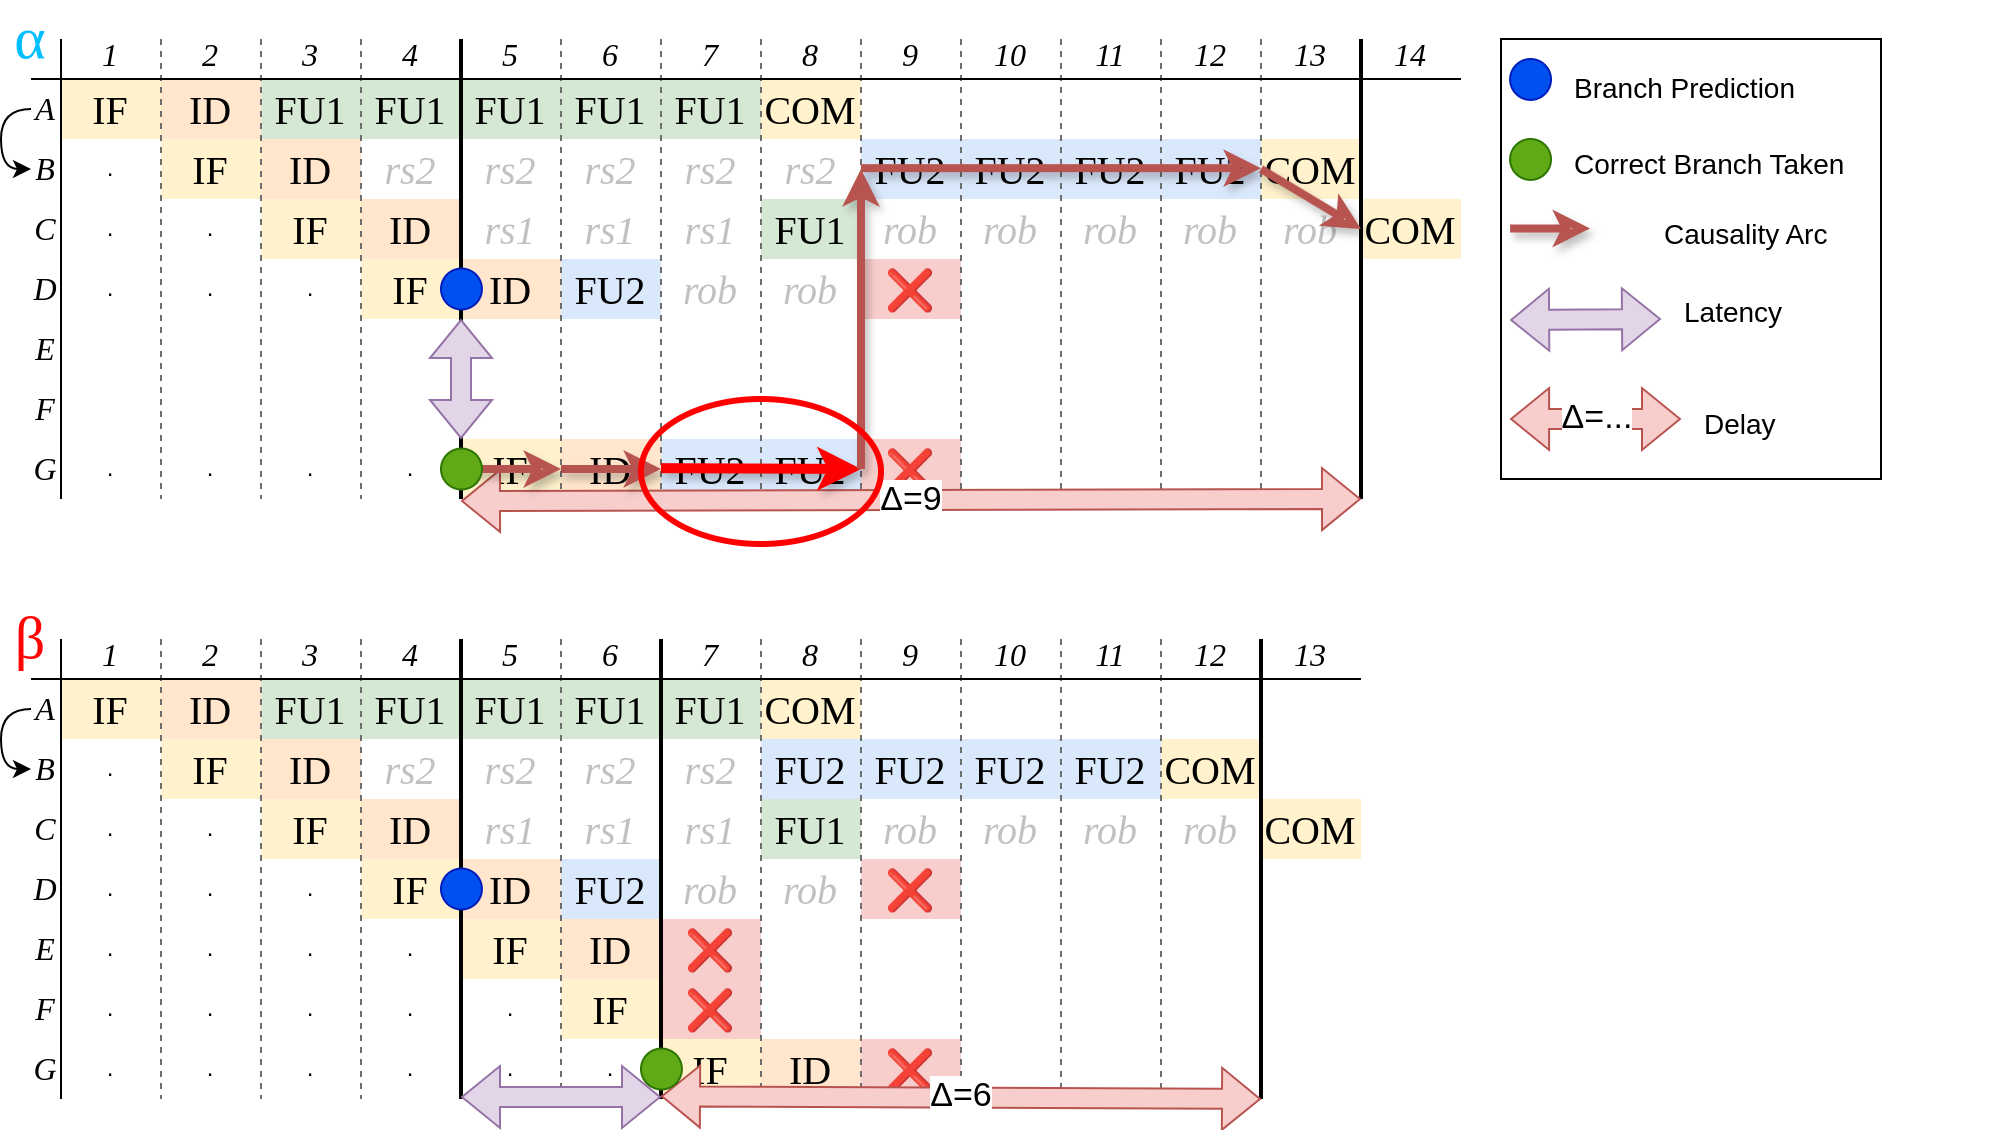
\includegraphics[width=\textwidth]{figures/nested-bp-ta.png}
    \caption{Execution trace of Example \ref{ex:nested-bp-ta}}
    \label{fig:nested-bp-ta-trace}
\end{figure}


In Figure \ref{fig:nested-bp-ta-trace}, we try to construct a causality graph for trace $\alpha$. In the picture, we show the causal path from the variation to the commit of $C$. However, one causal arc on the path (encircled in red) does not fit the definition: Remember that in Binder's definition, we have \textit{rule 4}, which creates an ETDG-arc $(\FUa \xrightarrow{lat_{FU}} \FUr)$. In Example \ref{ex:nested-bp-ta}, the FU-latency of $G$ is $4$; however, in trace $\alpha$, the delay between $\FUa_G$ and $\FUr_G$ is only $2$ clock cycles because of the earlier release of FU2 as a result of squashing. So, according to Binder's definition, the arc cannot be established and no TA exists.

Likely, we are just missing a rule that suffices to describe the anomaly here. Intuitively, $\FUr_G$ is caused by the squashing triggered by the branch resolution. Therefore, the $(\FUa_C \xrightarrow{0} \FUr_G)$ arc would make sense (Assumption \ref{ass:FU-squashing}). However, it does not allow us to construct a causality path in Example \ref{ex:nested-bp-ta} that can explain the TA happening.

\begin{assumption}
If FU is released as the result of squashing, the FU release of corresponding branch is causal to FU release of the squashed instruction.
\label{ass:FU-squashing}
\end{assumption}

Indeed, what we see in this example is that the earlier fetch of $G$ allows it to start executing, which prevents $B$ from starting the execution earlier. In fact, it is a reordering problem similar to Example \ref{ex:bp-ta}. For that reason we take an Assumption \ref{ass:FU-acq-rel} that effectively fills the gap in the causality path.

\TODO{why this is not a gap problem?}

\begin{assumption}
The FU acquisition is always causal to the respective FU release.
\label{ass:FU-acq-rel}
\end{assumption}

However, the following example shows that Assumption \ref{ass:FU-acq-rel} is not always correct. 

\begin{example}
\textbf{Latency Impact Through Misprediction Region}

We consider an instruction trace from Figure \ref{fig:lat-mispred-ta-input}; the pair of execution traces with TA is shown at Figure \ref{fig:lat-mispred-ta-trace}. Here the variation is in latency of $B$, but the effect propagates through the misprediction region of $F$ which consists of the instruction $G$. 
\label{ex:lat-mispred-ta}
\end{example}


\begin{figure}[H]
    \centering
    \begin{tabular}{rr|ccc}
    &  & Res. & Dep. & Lat. \\ \hline
    \textit{A:} &  & FU3 &  & $9$ \\
    \textit{B:} &  & FU1 &  & $6|7$ \\
    \textit{C:} &  & FU2 & $\{A, B\}$ & $4$ \\
    \textit{D:} &  & FU1 & $\{C\}$ & $4$ \\
    \textit{E:} &  & FU2 & $\{B\}$ & $4$ \\
    \textit{F:} &  & FU1 &  & $1$ \\
    & \textit{G:} & FU2 &  & $4$ \\
    \end{tabular}
    \caption{Instruction trace of Example \ref{ex:lat-mispred-ta}}
    \label{fig:lat-mispred-ta-input}
\end{figure}


\begin{figure}[H]
    \centering
    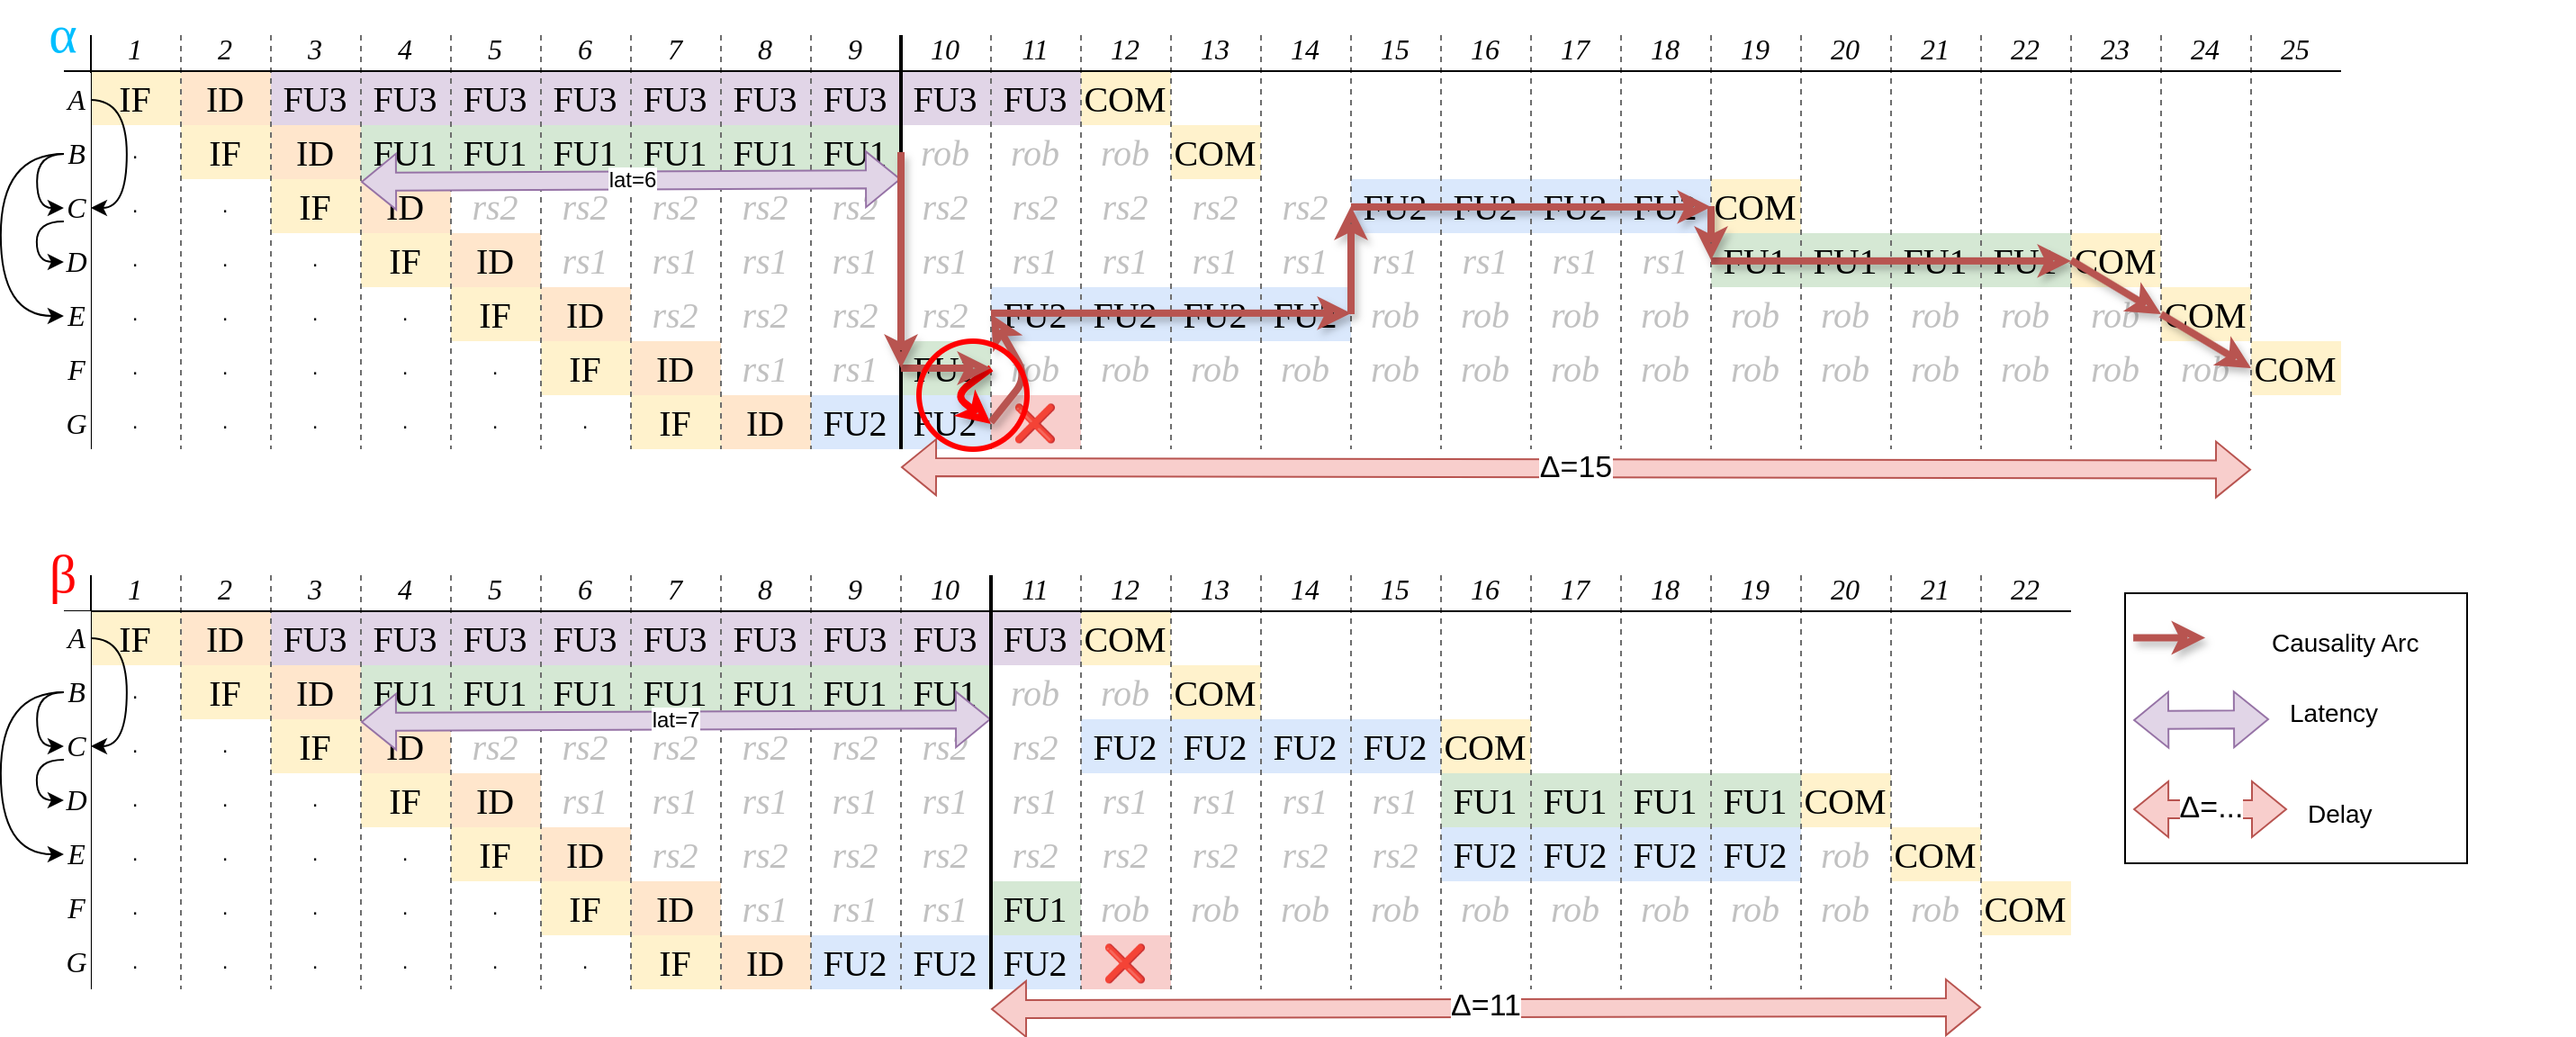
\includegraphics[width=\textwidth]{figures/lat-mispred.png}
    \caption{Execution trace of Example \ref{ex:lat-mispred-ta}}
    \label{fig:lat-mispred-ta-trace}
\end{figure}

Example \ref{ex:lat-mispred-ta} illustrates the problem with Assumption \ref{ass:FU-acq-rel}:  here if we try to draw a causality arc $(\FUa_G \xrightarrow{2} \FUr_G)$ in trace $\alpha$, the causality path can not build between $\FUr_B$ and $COM_E$. Instead, the Assumption \ref{ass:FU-squashing} works here allowing us to draw an arc $(\FUr_F \xrightarrow{0} \FUr_G)$.

\TODO{problem: consider only one trace}

\TODO{Conclusion: we need another definition}

\begin{example}
\textbf{Branch Prediction + Gap problem}

We modify Example \ref{ex:nested-bp-ta} by increasing latencies of instructions $A$ and $C$ by 2 (input trace in Figure \ref{fig:bp-gap-input}). This also requires us to define a larger misprediction region. The resulting pair of traces (Figure \ref{fig:bp-gap-trace}) exhibit a similar TA: instruction $J$ is fetched in trace $\alpha$ and postpones $B$.

\label{ex:bp-gap}
\end{example}

\begin{figure}[H]
    \centering
    \begin{tabular}{rrr|ccc}
    &  &  & Res. & Dep. & Lat. \\ \hline
    \textit{A:} &  &  & FU1 &  & $7$ \\
    \textit{B:} &  &  & FU2 & $\{A\}$ & $4$ \\
    \textit{C:} &  &  & FU1 &  & $1$ \\
    & \textit{*D:} &  & FU2 &  & $3$ \\
    &  & \textit{E:} & FU2 &  & $4$ \\
    &  & \textit{F:} & FU2 &  & $4$ \\
    &  & \textit{G:} & FU2 &  & $4$ \\
    &  & \textit{H:} & FU2 &  & $4$ \\
    & \textit{I:} &  & FU1 &  & $4$ \\
    & \textit{J:} &  & FU2 &  & $4$ \\
    \end{tabular}    

    \caption{Instruction trace of Example \ref{ex:bp-gap}}
    \label{fig:bp-gap-input}
\end{figure}

\begin{figure}
    \centering
    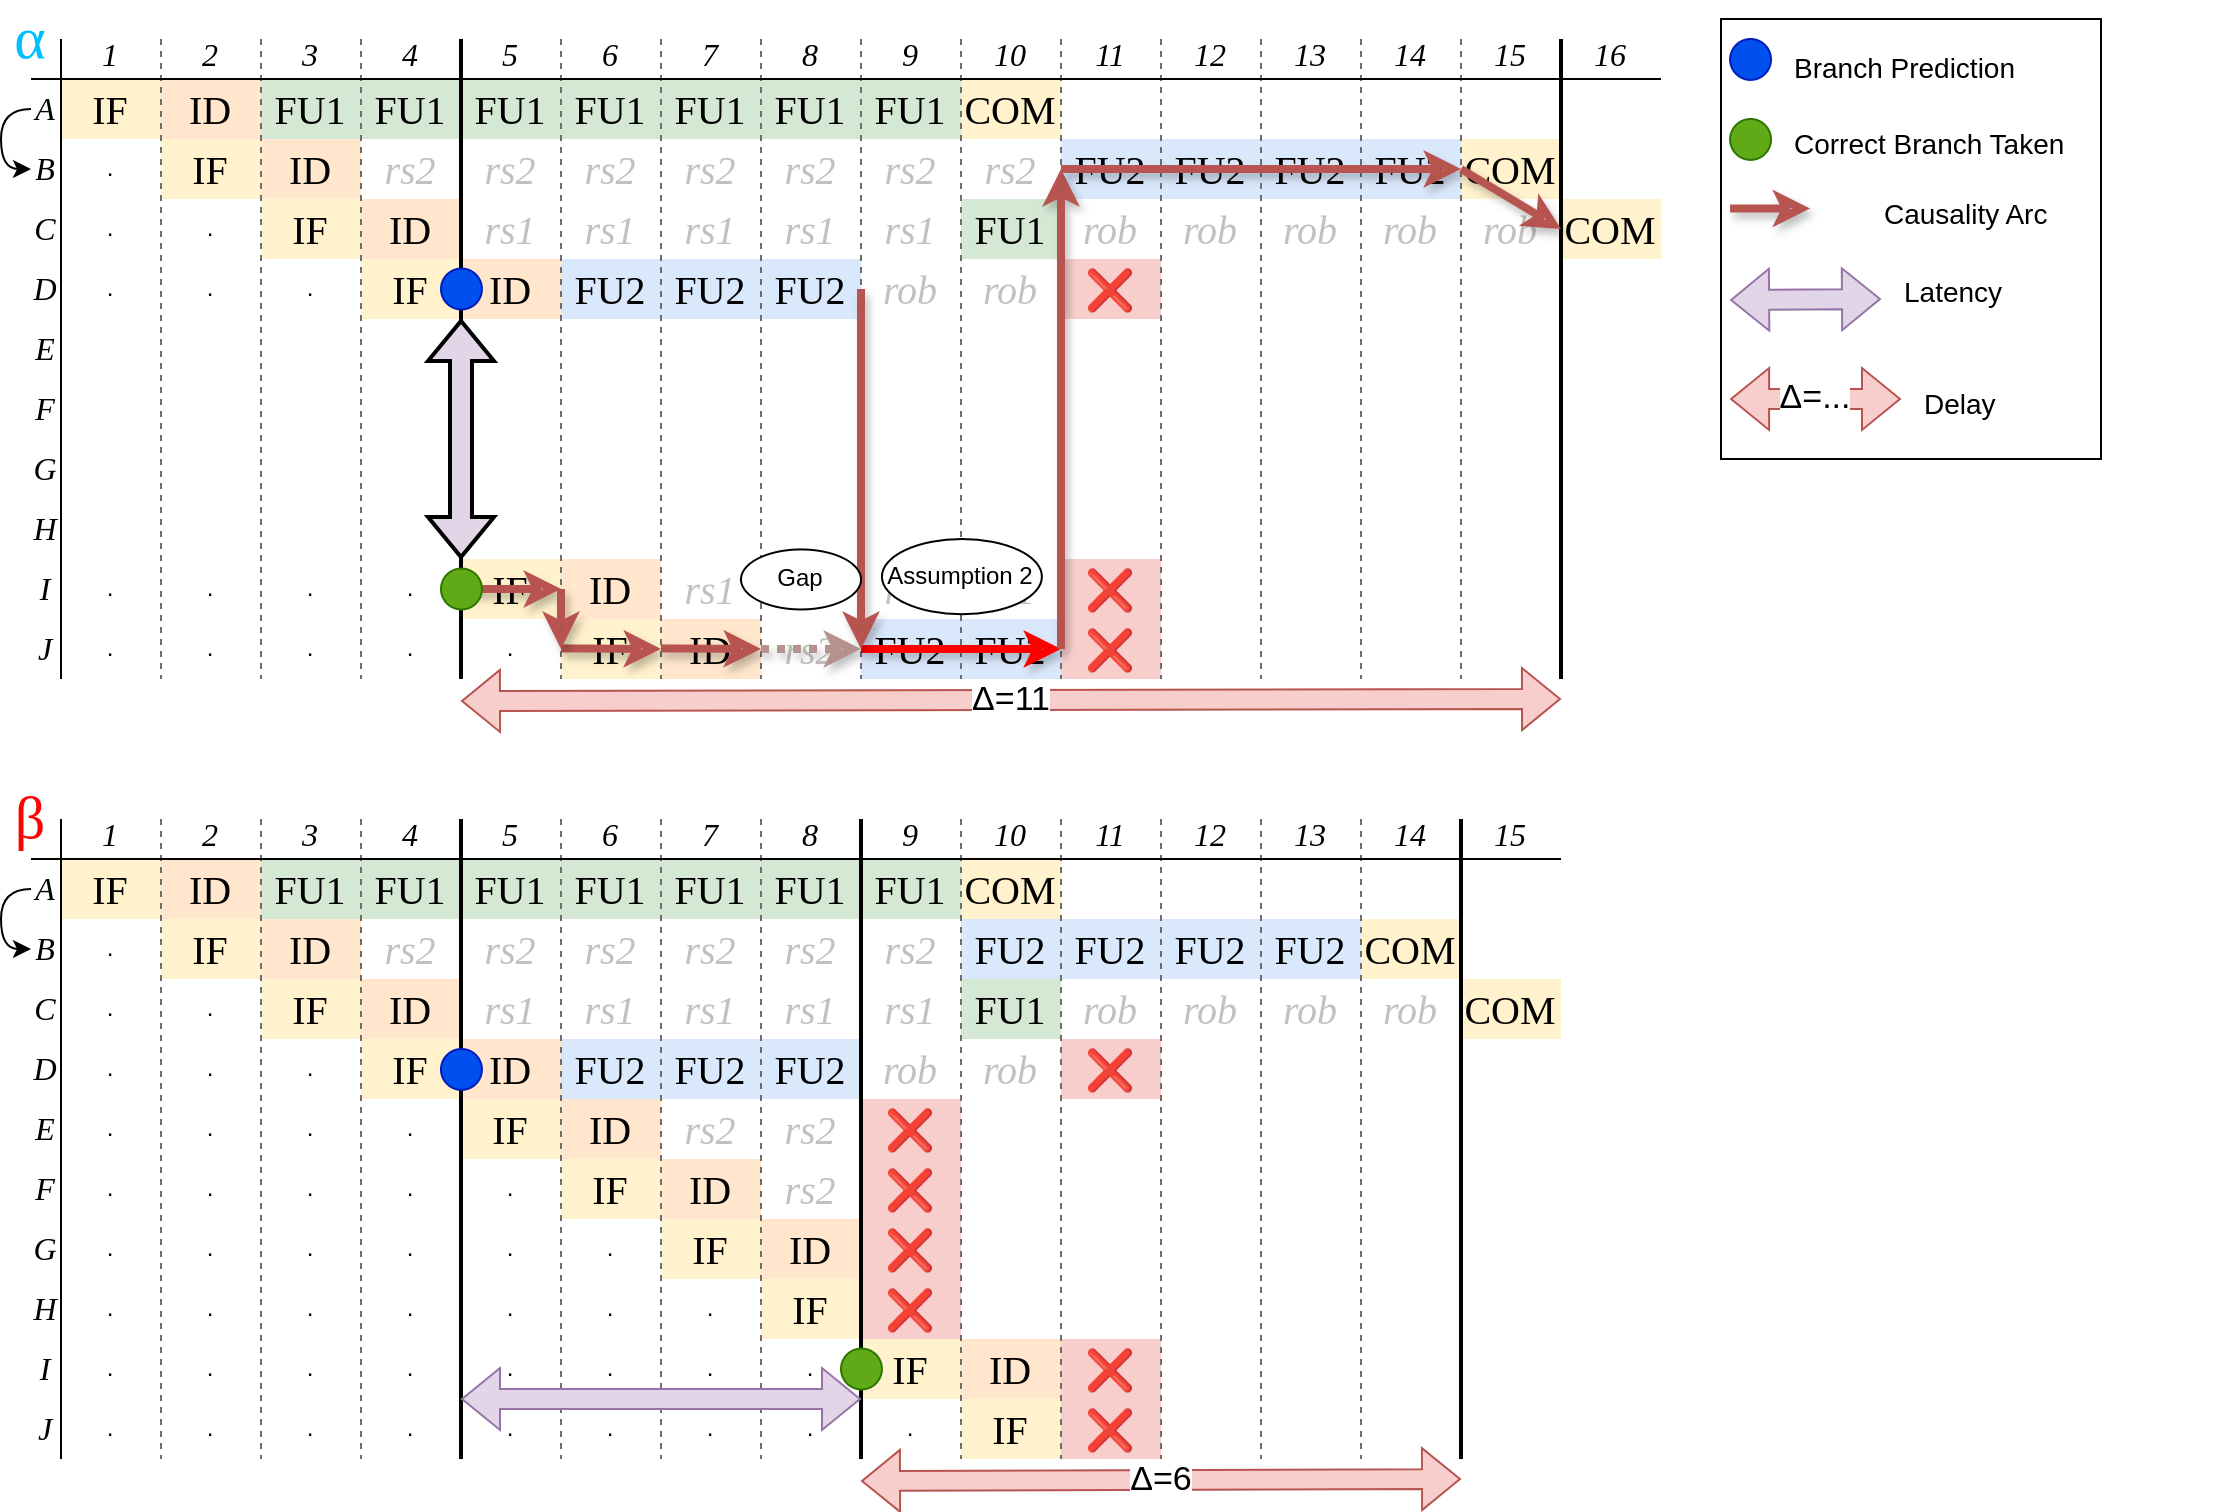
\includegraphics[width=\textwidth]{figures/bp-gap.png}
    \caption{Execution trace of Example \ref{ex:bp-gap}}
    \label{fig:bp-gap-trace}
\end{figure}

Example \ref{ex:bp-gap} shows that the gap problem can also arise in misprediction region. $\FUr_J$ in trace $\alpha$ is not detected as a part of causal region of the end of the variation $\IFa_I$ because of the resource contention rule which creates a stronger arc $(\FUr_D \xrightarrow{0} \FUa_J)$.

In summary, our analysis demonstrates that while the definition of Binder et al. shows promise for application to branch prediction scenarios, its adaptation requires the introduction of additional assumptions. However, the two assumptions we considered are mutually contradictory, precluding the formulation of a consistent and comprehensive definition. Furthermore, the original definition is susceptible to the gap problem, which also manifests in the context of branch prediction-induced timing anomalies.

We argue that these issues arise from fundamental limitations in the notion of causality adopted in Binder's work. Intuitively, causality should capture relationships such as "event $X$ was delayed due to event $Y$," but the current definition constructs causality arcs based solely on a single trace, without considering differences between traces. In Binder's framework, timing dependencies present in the trace with the unfavorable variation are disregarded, which is critical for understanding the propagation of timing anomalies. Both the gap problem and the contradictions between the proposed assumptions appear to originate from these conceptual shortcomings in the causality definition. Consequently, we believe that substantial revisions to the underlying notion of causality are necessary.


% Consequently, in the following section, we propose a novel approach to causality that aims to address these issues.

% \section{Towards New Causality Definition}

% TODO: formalize properties that we expect from causality graph and explain why they are violated

% TODO: propose a method that can be used to construct a "true causality" graph: set of constraints, moving events around